%Building
\documentclass[11pt]{article}

\usepackage[english]{babel}
\usepackage[margin=1in]{geometry}
\usepackage[colorlinks=true, allcolors=blue]{hyperref}

% Math/Greek packages
\usepackage{amssymb, amsmath, amsthm, mathtools, esint} 
\usepackage{algorithm, algorithmic}
\usepackage{upgreek}
\usepackage{physics}

% Graphics/Presentation packages
\usepackage{graphicx}
\usepackage{multirow, subcaption, cleveref}
\usepackage{tabulary, enumitem}
\usepackage{cancel}

%replace "ref" with "cref", "Cref", "crefrange"

% Misc packages
\renewcommand\qedsymbol{\textit{``Quack"}} %change the QED symbol to ``Quack" for the inside joke of Quantum Entangled Ducks

% defining where the images are
\graphicspath{ {../ESOF 322 Project (drive copy)/} }

\begin{document}

\title{ESOF 322: Project 1}
\author{Jake Coleman, William Jardee, Fletcher Philips, Megan Steinmasel}
\maketitle


%%TO-DO
% look for periods in usecase des
% check for any implementation in usecases
% remove website user from editing data
% add definition of eng/user



\textbf{General Feature}: \vspace{1.5em}

\noindent\textbf{User Story 1}:  As a website user, I want a functional navigation menu and search bar so that I can access information.\vspace{0.5em}

\noindent\textbf{User Story 3}: As a website user, I need the processing of new data to find important features and calculate relevant statistics to be done automatically, so it is friendly to someone that is not a data scientist.\vspace{0.5em}

\noindent\textbf{User Story 4}: As a website user, I want a data visualization technique that is intuitive and accurately shows patterns in the data.\vspace{0.5em}

\noindent\textbf{User Story 5}: As a database engineer, I want to have a database so that I can store cold cases inside of it. \vspace{0.5em}

\noindent\textbf{User Story 6}: As a database engineer, I want the data to be manipulatable so that the admin can insert and delete data from the database.\vspace{0.5em}



%--------------------------------------------------------------------
%Visualize Results
%--------------------------------------------------------------------
\begin{table}[!ht]
\begin{center}
\textbf{Author: Jake Coleman}
\vspace*{1em}

\begin{tabular}{p{0.30\linewidth}p{0.60\linewidth}}
	Name: & Visualize Results\\\hline
	Description: & Displays selected graphs from the gathered data\\\hline
	Related Requirements:& User Story 2\\\hline
	Preconditions:& The website user has signed into the website and accessed the drop-down menu to access the page. Some data has been selected for an analysis and the desired type of graph has been selected.\\\hline
	Successful end condition:& The graphs are displayed on a separate page to view.\\\hline
	Failed end condition:& Fails to display any graphs\\\hline
	Actors:& Website User\\\hline
	Basic Flow of Events: & \begin{enumerate}
	\item The website user goes through the drop-down menu process
	\item The website user chooses to view graphs via drop-down menu
	\item The system will display any applicable graphs
	\end{enumerate}\\\hline
	Extensions/Exceptional Flow of Events & \begin{enumerate}
	\item The graphs fail to display
	\item the User is notified that the use is unable to access graphs via a notification
	\item write to log file
	\item User is sent back to main navigation system
	\end{enumerate}
\end{tabular}
\label{des:vis_res}	
\end{center}
\end{table}
%--------------------------------------------------------------------


%--------------------------------------------------------------------
%Create Database
%--------------------------------------------------------------------
\begin{table}[!ht]
\begin{center}
\textbf{Author: Fletcher Philips}
\vspace*{1em}

\begin{tabular}{p{0.30\linewidth}p{0.60\linewidth}}
	Name: & Create Database\\\hline
	Description: & A database needs to be created and connected to the web framework we choose\\\hline
	Related Requirements:& User Story 5\\\hline
	Preconditions:& Basic web infrastructure has been created. Small sample set of cold cases is ready to be inserted.\\\hline
	Successful end condition:& Basic database has been initialized with substructure. Data has been inserted into the database.\\\hline
	Failed end condition:& Data cannot be inserted into the database.\\\hline
	Actors:& Database engineer\\\hline
	Basic Flow of Events: & \begin{enumerate}
	\item Create MySQL Database.
	\item Connect a database to the web framework
	\item Insert Data into MySQL database
	\end{enumerate}\\\hline
	Extensions/Exceptional Flow of Events & \begin{enumerate}
	\item Database fails to build properly
	\item the engineer is notified that an error has appeared
	\item write to log file
	\item engineer is ejected from the system
	\end{enumerate}
\end{tabular}
\label{des:create_database}	
\end{center}
\end{table}
%--------------------------------------------------------------------


%--------------------------------------------------------------------
%Connects to Web
%--------------------------------------------------------------------
\begin{table}[!ht]
\begin{center}
\textbf{Author: }
\vspace*{1em}

\begin{tabular}{p{0.30\linewidth}p{0.60\linewidth}}
	Name: & \\\hline
	Description: & \\\hline
	Related Requirements:& \\\hline
	Preconditions:& \\\hline
	Successful end condition:& \\\hline
	Failed end condition:& \\\hline
	Actors:& \\\hline
	Basic Flow of Events: & \begin{enumerate}
	\item .
	\end{enumerate}\\\hline
	Extensions/Exceptional Flow of Events & \begin{enumerate}
	\item .
	\end{enumerate}
\end{tabular}
\label{des:con_web}	
\end{center}
\end{table}
%--------------------------------------------------------------------


%--------------------------------------------------------------------
%Manage Data
%--------------------------------------------------------------------
\begin{table}[!ht]
\begin{center}
\textbf{Author: William Jardee}
\vspace*{1em}

\begin{tabular}{p{0.30\linewidth}p{0.60\linewidth}}
	Name: & Manage Data\\\hline
	Description: & Data needs to be inserted, deleted, and manipulated. Related to this, there must be an appropriate Graphical User Interface. The data will connect directly with the database.\\\hline
	Related Requirements:& User Story 3, User Story 6\\\hline
	Preconditions:& The user is logged on and has gained access rights according to their credentials.\\\hline
	Successful end condition:& Data is successfully manipulated and success code received from source. \\\hline
	Failed end condition:& Requested task is outside of credentials. Success code not received. Invalid new data\\\hline
	Actors:& Website User, Database engineer\\\hline
	Basic Flow of Events: & \begin{enumerate}
	\item Actor selects the action they wish to commit, and what to commit it on.
	\item Action is tested against credentials
	\item Success/Fail state is determined
	\item any follow-up effects happen (i.e., Visualize Results Via Graph)
	\item Flow is complete and prompts user for next action
	\end{enumerate}\\\hline
	Extensions/Exceptional Flow of Events & \begin{enumerate}
	\item Conflict happens
	\item Reject any attempted changes and revert to the last viable state
	\item Notify actor that there has been an error and write to log file
	\item Flow is complete and prompts user for next action
	\end{enumerate}
\end{tabular}
\label{des:man_dat}	
\end{center}
\end{table}
%--------------------------------------------------------------------



%--------------------------------------------------------------------
%Creaete Log
%--------------------------------------------------------------------
\begin{table}[!ht]
\begin{center}
\textbf{Author: William Jardee}
\vspace*{1em}

\begin{tabular}{p{0.30\linewidth}p{0.60\linewidth}}
	Name: & Create Log\\\hline
	Description: & A log file should be kept to keep track of flow as to diagnose errors and suspicious behavior.\\\hline
	Related Requirements:& Catch all location for all errors\\\hline
	Preconditions:& The system has been started effectively and there is a safe place to store a text file (log file).\\\hline
	Successful end condition:& Data can be saved to the log file\\\hline
	Failed end condition:& Data cannot be safely save to log file\\\hline
	Actors:& Database engineer \\\hline
	Basic Flow of Events: & \begin{enumerate}
	\item Write to file recent activity
	\item Flag any invalid actions that prompt ``write to log file"
	\end{enumerate}\\\hline
	Extensions/Exceptional Flow of Events & \begin{enumerate}
	\item Notify system admin of issue and include error information
	\item Terminate all systems until issue is resolved
	\end{enumerate}
\end{tabular}
\label{des:create_log}
\end{center}
\end{table}
%--------------------------------------------------------------------


\begin{figure}[!ht]
\centering
	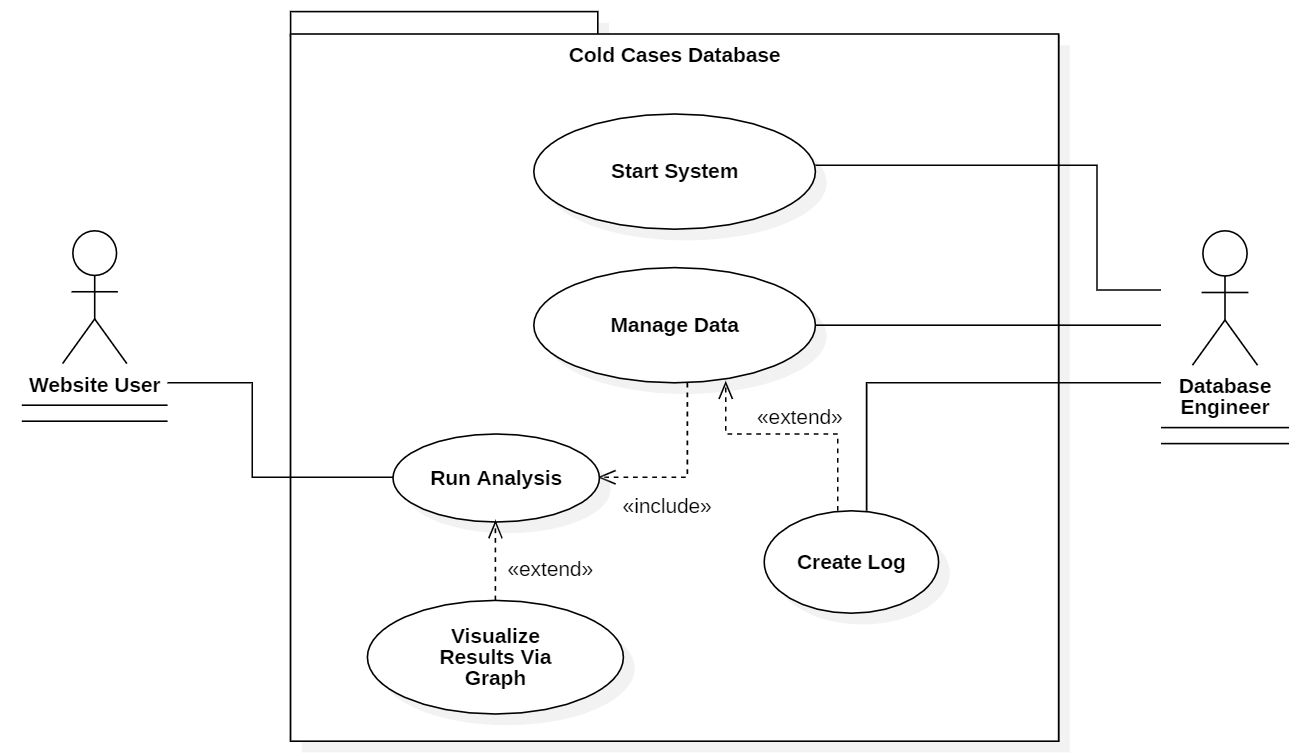
\includegraphics[width=.95\textwidth]{./UseCases/jardee_usecase}\\
	\caption{UseCase diagram for the Cold-Cases Database system.}
	\label{fig:usecase_diagram}
\end{figure}
\clearpage

\begin{figure}[!ht]
\centering
	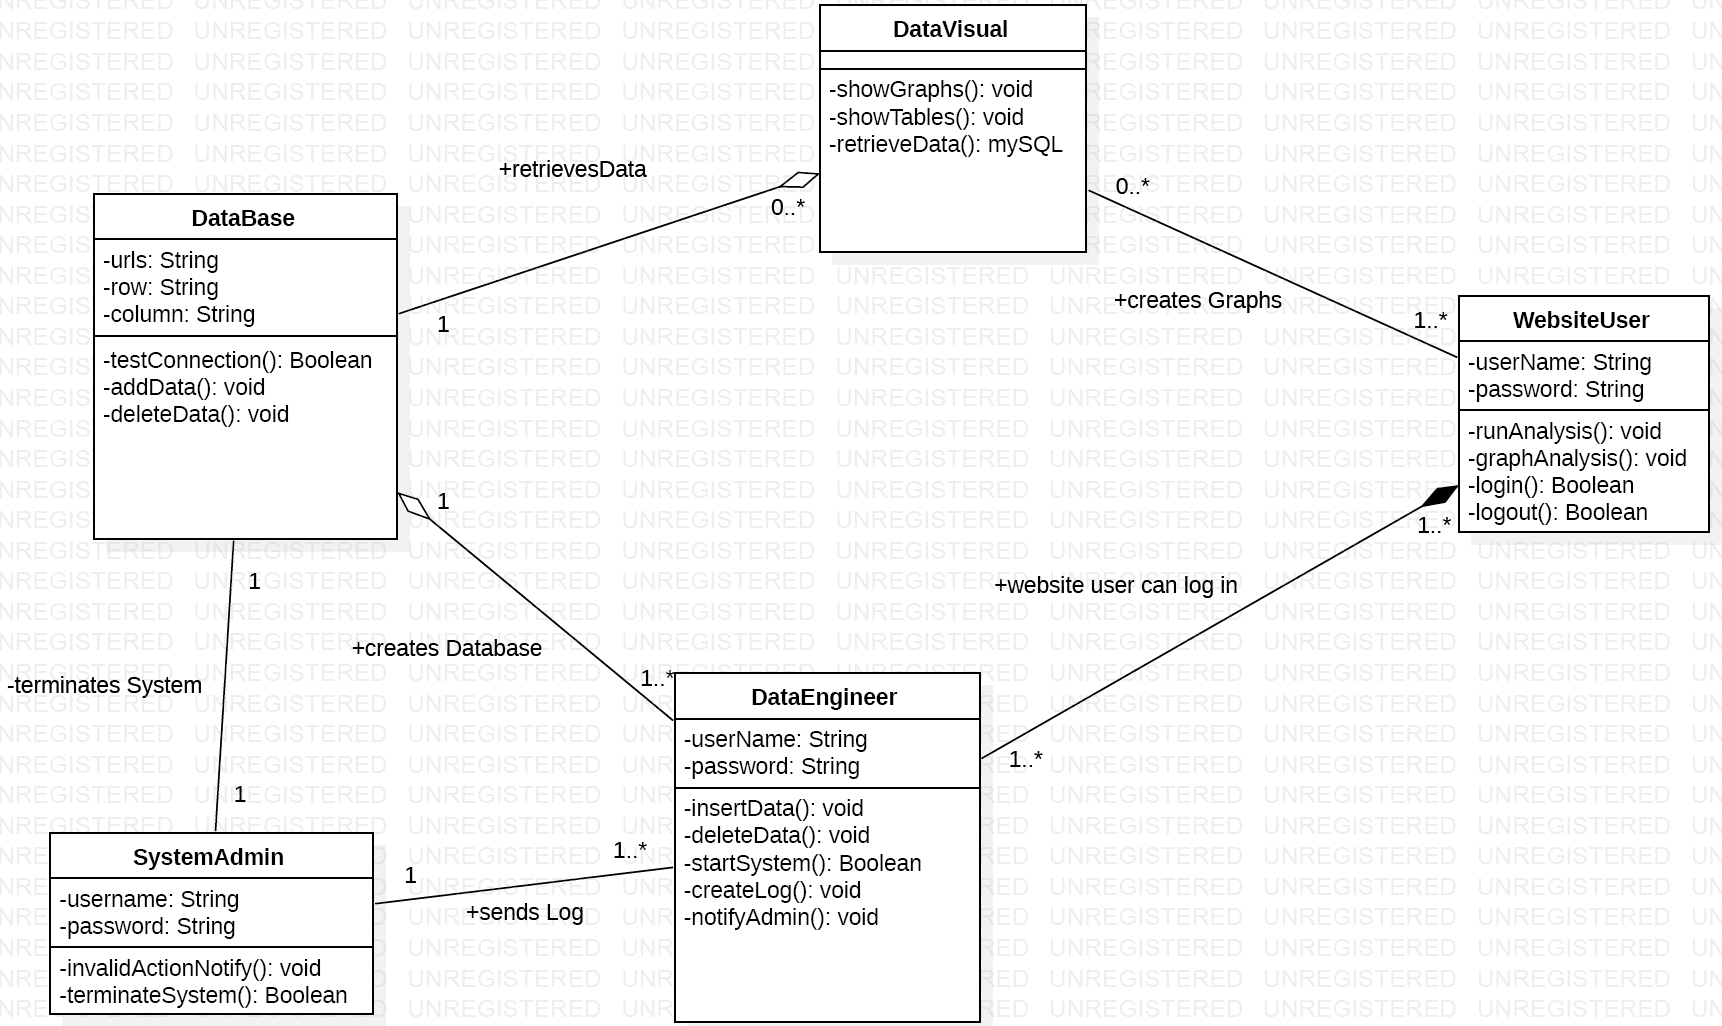
\includegraphics[width=.95\textwidth]{./Class Diagrams/ColdCaseClassDiagram}\\
	\caption{Class diagram for the Cold-Cases Database system.}
	\label{fig:class_diagram}
\end{figure}
\clearpage

\begin{figure}[!ht]
\centering
	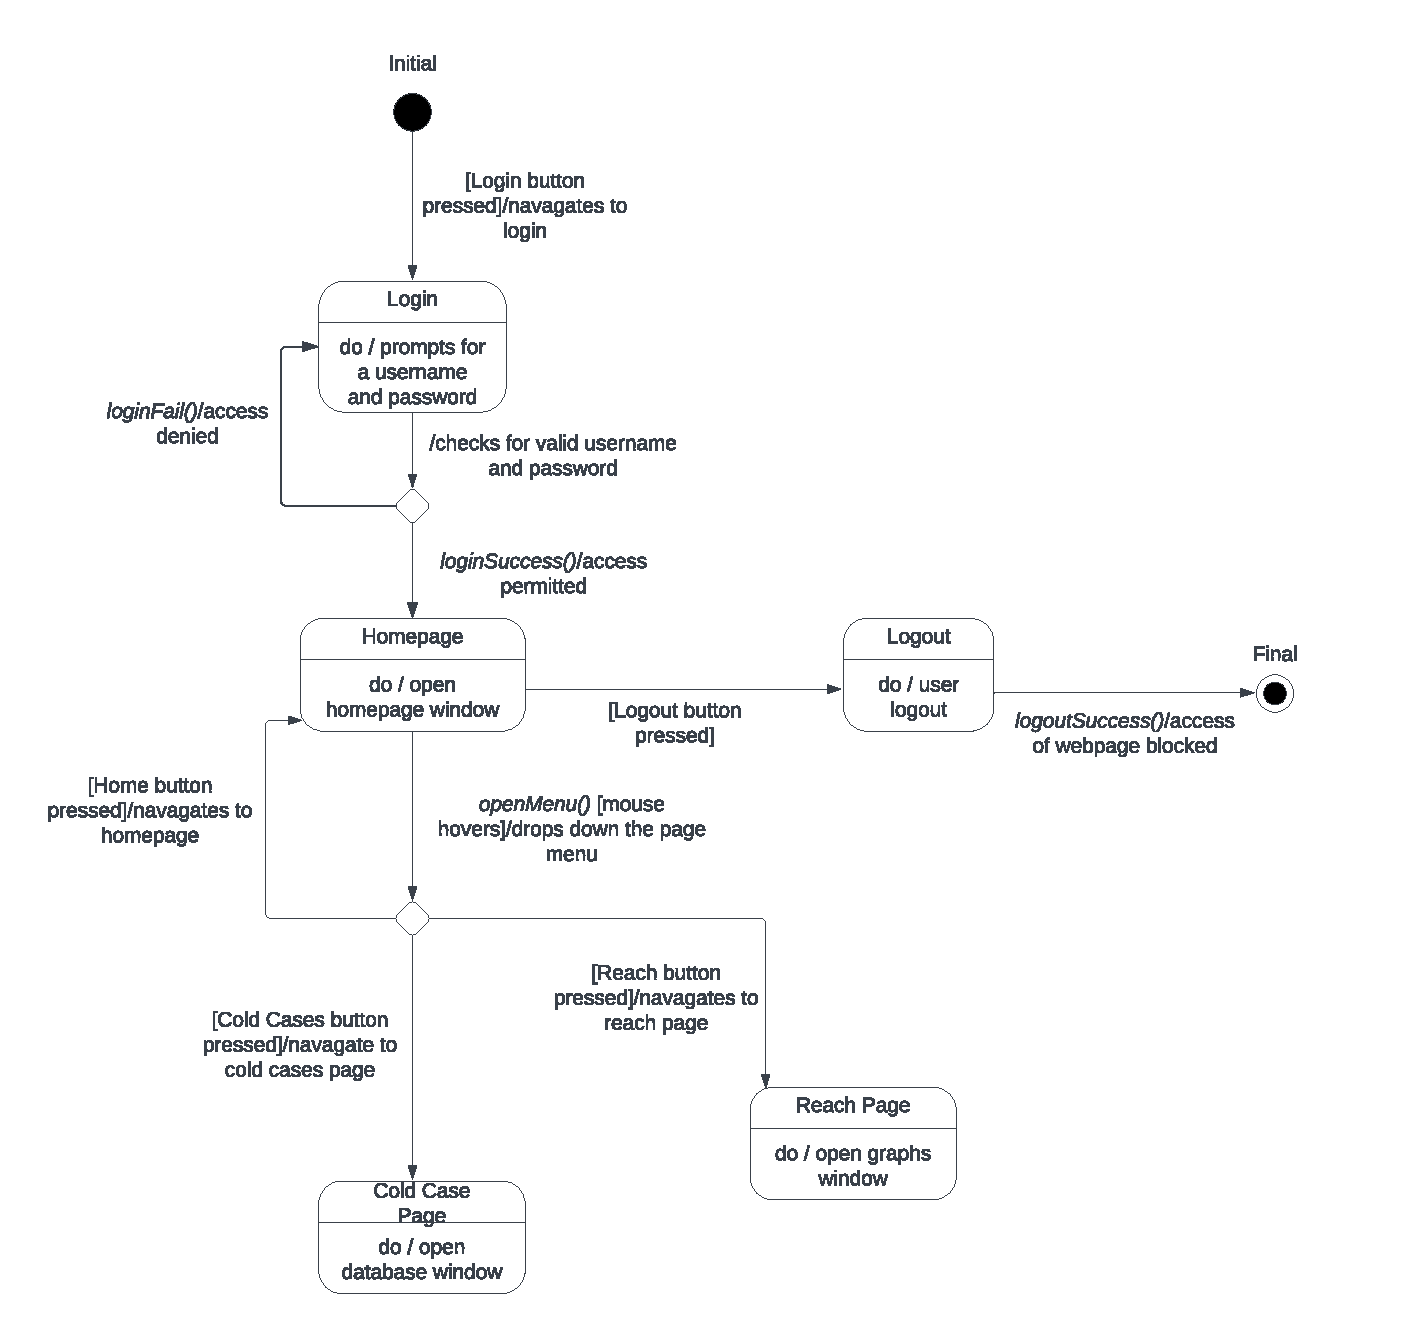
\includegraphics[width=.95\textwidth]{./State Chart/C.C. Statechart}\\
	\caption{State Chart diagram for the Cold-Cases Database system.}
	\label{fig:state_chart_diagram}
\end{figure}
\clearpage

\begin{figure}[!ht]
\centering
	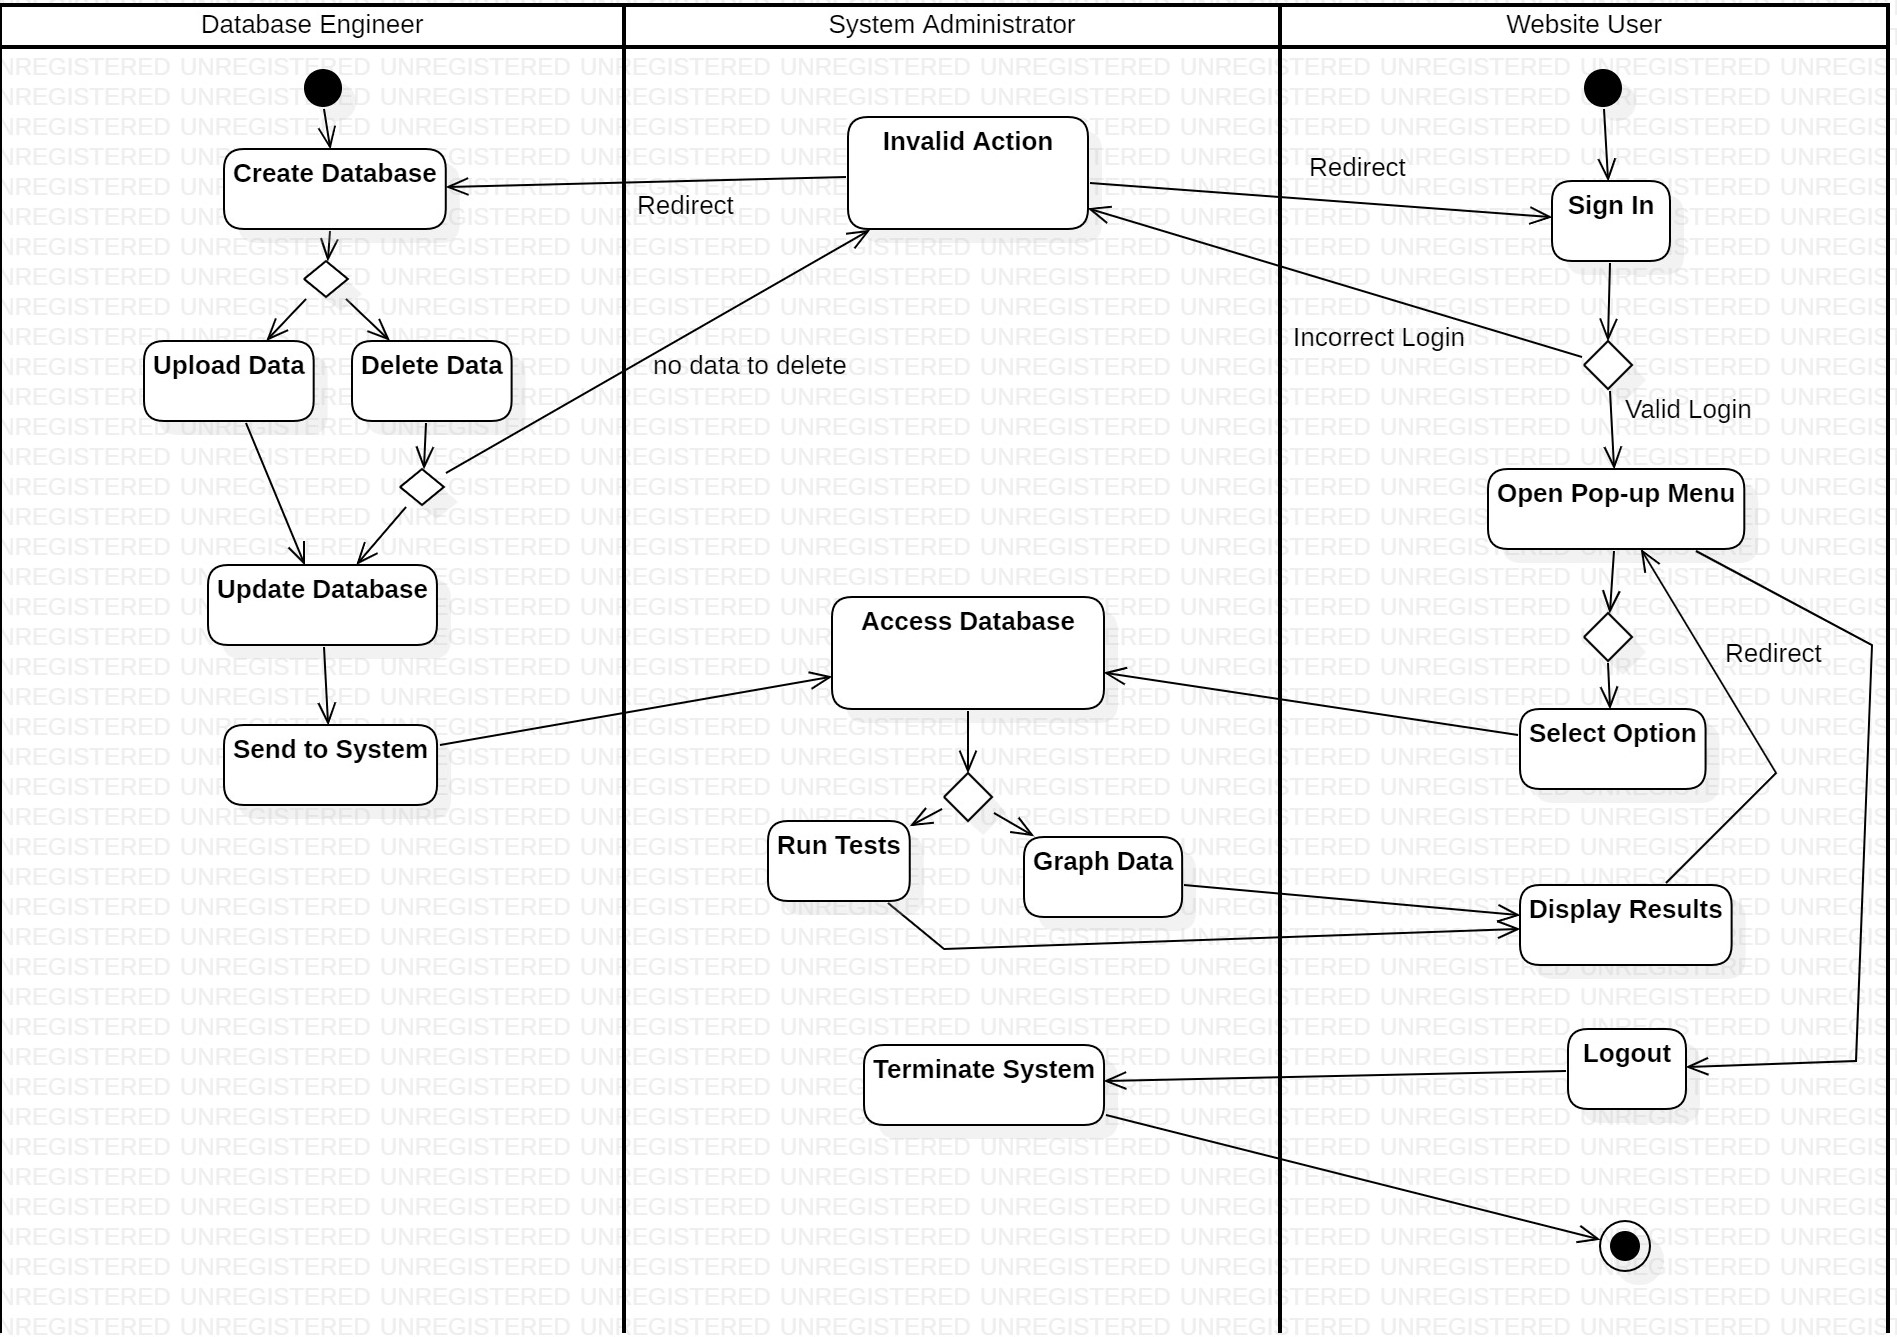
\includegraphics[width=.95\textwidth]{./Activity Diagram/activitydiagram2}\\
	\caption{Activity diagram for the Cold-Cases Database system.}
	\label{fig:activity_diagram}
\end{figure}
\clearpage


\end{document}
